\documentclass[11pt, spanish]{article}
\usepackage[spanish]{babel}
\selectlanguage{spanish}
\usepackage[utf8]{inputenc}
\usepackage{graphicx}
\usepackage{mathtools}
\usepackage{tabularx}
\usepackage[font=small,labelfont=bf]{caption}
\usepackage{subcaption}
\usepackage{authblk}
\usepackage{natbib}

\captionsetup[table]{name=Tabla}
\renewcommand{\thetable}{\Roman{table}}
\newcommand{\mean}[1]{\left\langle#1\right\rangle}
%\newcommand{\eqref}[1]{Ec.~\ref{#1}}

\begin{document}
\begin{titlepage}
    \centering
    {\scshape\LARGE Universidad de Buenos Aires \par}
    \vspace{1cm}
    {\scshape\Large Informe 1\par}
    \vspace{1.5cm}
    {\huge\bfseries Redes Complejas\par}
    \vspace{2cm}
    {\Large\itshape Ra\'ul Barriga\par}
    {\Large\itshape Mariela Celis\par}
    {\Large\itshape Jimmy Mas\'ias\par}
    {\Large\itshape Sebast\'ian Pinto\par}

    \vfill

    \vfill

                                                    % Bottom of the page
    {\large \today\par}
\end{titlepage}
    %\input{intro}

\tableofcontents

\newpage

\section{Ejercicio 1}

Se consideran tres redes de interacci\'on prote\'inas de levadura: Red de 
copertenencia a complejos proteicos (AP-MS); Red de interacciones binarias 
(Y2H); y una red obtenida de la literatura (LIT), todas obtenidas del 
\textit{Yeast Interactome Database}, y mostradas en la figura \ref{fig:ej1_grafos}.

\begin{figure}[!ht]
    \centering
    \begin{subfigure}[b]{0.40\columnwidth}
        \includegraphics[width=\textwidth]{./schemes/yeast_AP-MS.pdf}
        \caption{\label{fig:ap_ms} AP-MS}
    \end{subfigure}
    \begin{subfigure}[b]{0.40\columnwidth}
        \includegraphics[width=\textwidth]{./schemes/yeast_LIT.pdf}
        \caption{\label{fig:LIT}LIT}
    \end{subfigure}
    \\
    \begin{subfigure}[b]{0.40\columnwidth}
        \includegraphics[width=\textwidth]{./schemes/yeast_Y2H.pdf}
        \caption{\label{fig:y2h} Y2H}
    \end{subfigure}
    \caption{\label{fig:ej1_grafos} Esquematizaci\'on de los grafos de cada 
    red estudiada. Se utiliz\'o un \textit{layout} estilo Frunchterman-Reigold 
    para la representaci\'on.}
\end{figure}

Graficamente se puede observar que la red Y2H tiene un nucleo bien definido
y un gran n\'umero de nodos conectados a \'el, esto significa que es posible
diferenciar dos grupos proteicos: Mediadoras (interaccionan con un gran
n\'umero de prote\'inas) y Mediadas (realizan alg\'un tipo de funci\'on con
ayuda de las mediadoras). El grupo de las Mediadoras (Nucleo) es probable 
que est\'e formado exlusivamente por enzimas.

Por otro lado en grafo AP-MS se pueden observar peque\~nos nucleos/clusters
muy conectados entre si y menos conectados con el resto. Estos nucleos dispersos
por la red son los complejos proteicos que busca carecterizar la red. 

\textbf{Que decir de la red LIT ??}\\


Una caracterizacion global y cuantitativa de las redes se muestra en la 
Tabla~\ref{tab:obs}. En ella se muestran diferentes observables globales
\textbf{Son realmente dirigidas ? analisis simple pero se debe tener claro
si se est\'a analizando lo correcto\ldots}
\begin{table}[!ht]
    \centering
    {\scriptsize
    \begin{tabularx}{1\columnwidth}{XlX|XcXcXcX}
        \hline\hline
        &Observables        &&& AP-MS && LIT && Y2H &\\ 
        \hline
        &Red dirigida       &&& Si && Si && Si &\\
        &Tiene loops        &&& No && Si && Si &\\
        &N$^o$ nodos $N$    &&& 1622 && 1536 && 2018 &\\
        &N$^o$ enlaces $L$  &&& 9070 && 2925 && 2930 &\\
        &Densidad           &&& 0.0034 && 0.0014 && 0.0007 &\\
        &Diametro           &&& 10 && 8 && 11 &\\
        \hline
        &Grado in $k_{in}$&&&\\
  %      \hline
        &\quad medio  $\mean{k_{in}}$     &&& 5.59 && 1.90 && 1.45 &\\
        &\quad maximo $\max(\{k_{in}\})$  &&& 111  && 23   && 66 &\\ 
        &\quad minimo $\min(\{k_{in}\})$  &&& 0    && 0    && 0 &\\ 
        \hline
        &Grado in $k_{out}$&&&\\
 %       \hline
        &\quad medio  $\mean{k_{out}}$     &&& 5.59 && 1.90 && 1.45 &\\
        &\quad maximo $\max(\{k_{out}\})$  &&& 85   && 35   && 38   &\\ 
        &\quad minimo $\min(\{k_{out}\})$  &&& 0    && 0    && 0    &\\ 
        \hline
        &Coeficiente de Clusterizaci\'on&&&\\
%        \hline
        &\quad medio/local $\mean{C}$               &&& 0.0741 && 0.4556 && 0.0970 & \\
        &\quad triangular/global $C_\bigtriangleup$ &&& 0.6185 && 0.3461 && 0.0236 & \\
        \hline\hline
    \end{tabularx}
    }
    \caption{\label{tab:obs}Observables para las tres redes de interacci\'on prote\'ica de levadura.}
\end{table}
        
    
\textbf{Diagrama de venn ???}

\newpage

\section{Ejercicio 2.}

\subsection{Parte a.}

\par Exploramos diferentes layouts para visualizar la red delfines.
En la figura \ref{fig:Layout_delfines} observamos el resultado de graficar
el grafo con el Fruchterman - Reingold layout. 
\par El algoritmo para realizar este layout se basa en asignarles fuerzas de interacción ficticias a los nodos. Típicamente se basa en que los nodos ligados tengan una fuerza de atracción análoga a la fuerza de un resorte, sumado a una fuerza de repulsión entre todos los nodos, análoga a la interacción coloumbiana entre partículas cargadas idénticamente.
\par Este tipo de layout nos permitió visualizar la existencia de dos comunas de delfines, ligadas a través de unos pocos nodos.

\begin{figure}[h]
\centering
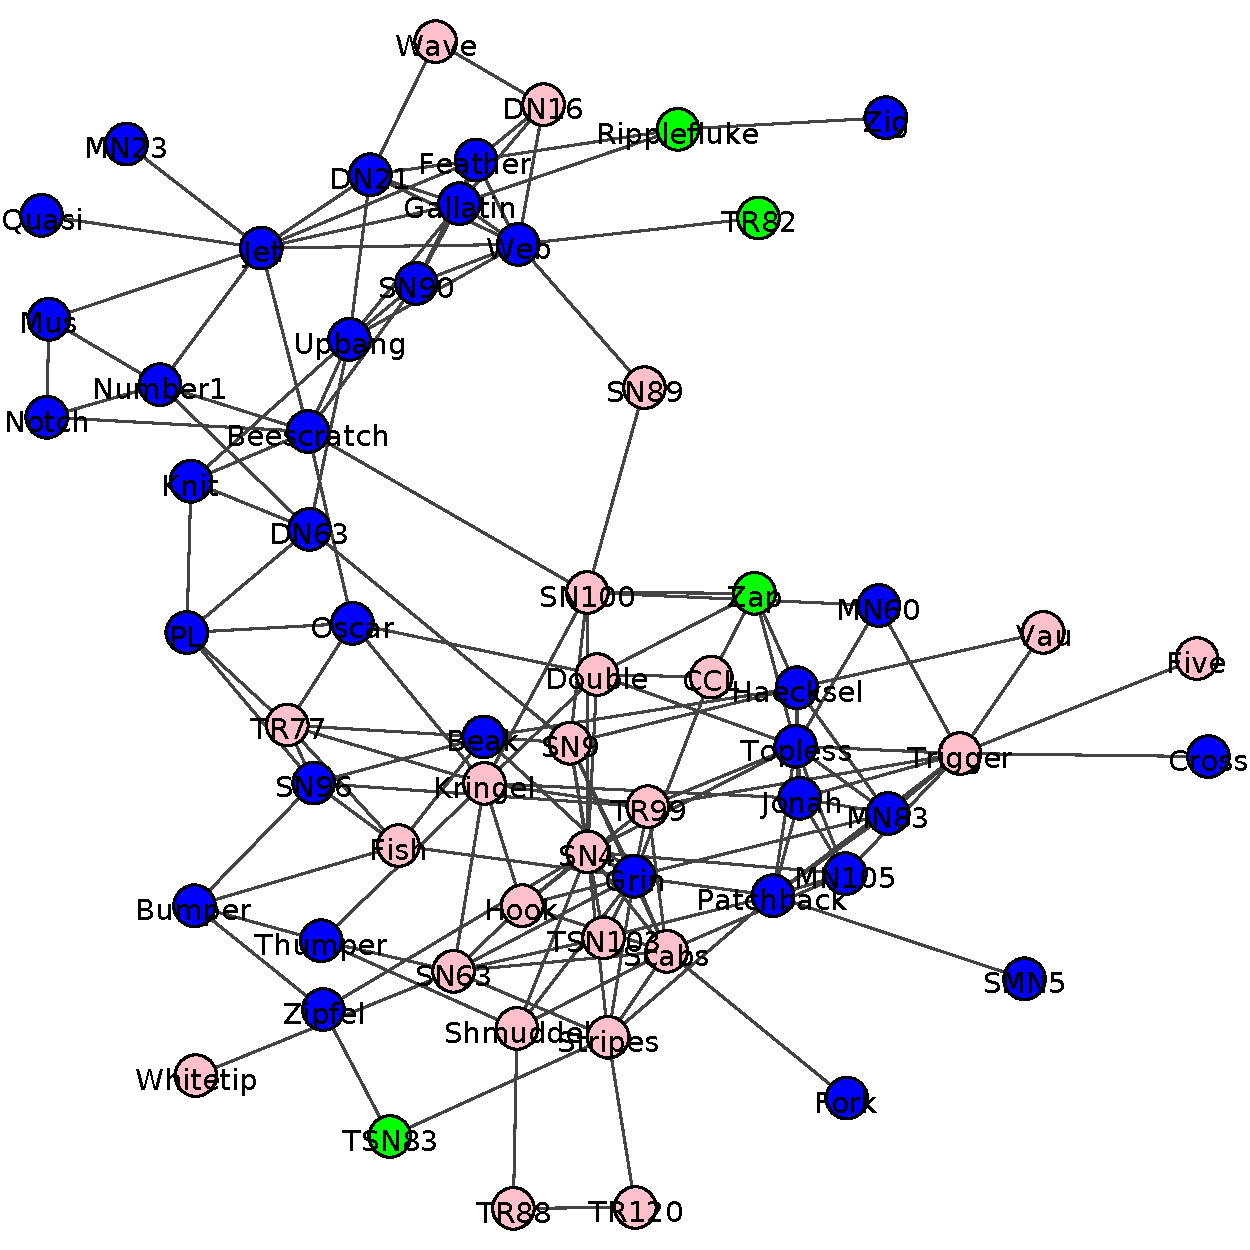
\includegraphics[scale = 0.50]{figuras/FrutRein}
\label{fig:Layout_delfines}
\caption{Fruchterman - Reingold layout. Los colores de los nodos se refieren al sexo del delfín: azul, macho; rosa, hembra; verde, sexo no indicado en el dataset.}
\end{figure}

\subsection{Parte b.}

\par En esta sección nos propusimos estudiar si la red era de carácter homofílica o no, es decir, si un dado nodo tiende a ligarse con nodos que comparten una caractrística con él, como es en este caso, el género de los delfines.
Para ello, se comparó la red de delfines con el género asociado con una red de misma topología pero sorteando al azar el género de los delfines. Esto constituye lo que llamamos hipótesis nula, es decir, el género de un delfín es asignado de manera totalmente independiente a la topología de la red.
\par En la red del dataset, la fracción de links entre delfines de distinto género (sin contar los pares de vértices que incluyan un delfín con género no especificado) es de $\rho_{M-F} \sim 0.32$. Manteniendo constante la topología de la red sorteamos los géneros entre los nodos, manteniendo constante la cantidad de machos, hembras, y ejemplares sin especificación de genero. Realizamos $1000000$ de realizacion, calculando la fracción de links entre géneros al final, obteniendo como resultado el histograma de la figura \ref{fig:Histograma}.
\par El valor medio de links entre géneros de la distribución obtenida es $<\rho_{M-F}>^{HN} = 0.43 \pm 0.04$, donde el error es la desviación estandar de la misma.
\par Del histograma podemos concluir que, dada la hipotesis nula, la probabilidad de que la fracción de links entre géneros sea $\sim 0.32$ es menor a $0.005$, por lo que podemos descartar la hipótesis nula, es decir, la distribución actual de links entre géneros no proviene de una distribución al azar de los mismos. Por otro lado, este número es mucho menor que el valor medio $<\rho_{M-F}>^{HN}$, lo cual indica que la mayor cantidad de links se da entre delfines del mismo género, lo cual apoya la hipótesis de que esta red es homofílica.
\par Estimación del valor medio: la probabilidad de tomar un link entre un macho y una hembra es $2 \rho_{M} \rho_{F}$, donde $\rho$ son las densidades de cada género en la red real. Entonces la probabilidad de la tomar $m$ links es:
\begin{equation}
	P(m) = {N' \choose m} (2 \rho_{M} \rho_{F})^{m} (1 - 2 \rho_{M} \rho_{F})^{N' - m}
\end{equation}
donde $N'$ es $N(N-1)/2$, el número total de links que se pueden formar en una red de $N$ nodos. El valor medio de links es entonces $<m> = N' 2 \rho_{M} \rho_{F}$, y la desviación estándar de links $std(m) = (N' 2 \rho_{M} \rho_{F} (1 - 2 \rho_{M} \rho_{F}))^{1/2}$. Para los valores del problema, obtenemos:
\begin{equation}
	<m> = 68 \pm 7 
\end{equation}

\begin{tabbing}
\hspace{5cm} \= \hspace{5cm} \kill
Observable \> Valor \\
$N$ \> $62$ \\
$N' = N(N-1)/2$ \> $1891$ \\
$\rho_{M}$ \> $0.55$ \\
$\rho_{F}$ \> $0.39$ \\
$p_{M-F}$ \> $2 \rho_{M} \rho_{F} \sim 0.43 $ \\
$<m>_{estimado}$ \> $N' p_{M-F} \sim 811$
\end{tabbing}



\begin{figure}[h]
\centering
\includegraphics[scale = 0.50]{figuras/Histograma}
\label{fig:Histograma}
\caption{Histograma}
\end{figure}

\subsection{Parte c.}

\begin{figure}
\centering
\begin{subfloat}[]
{
	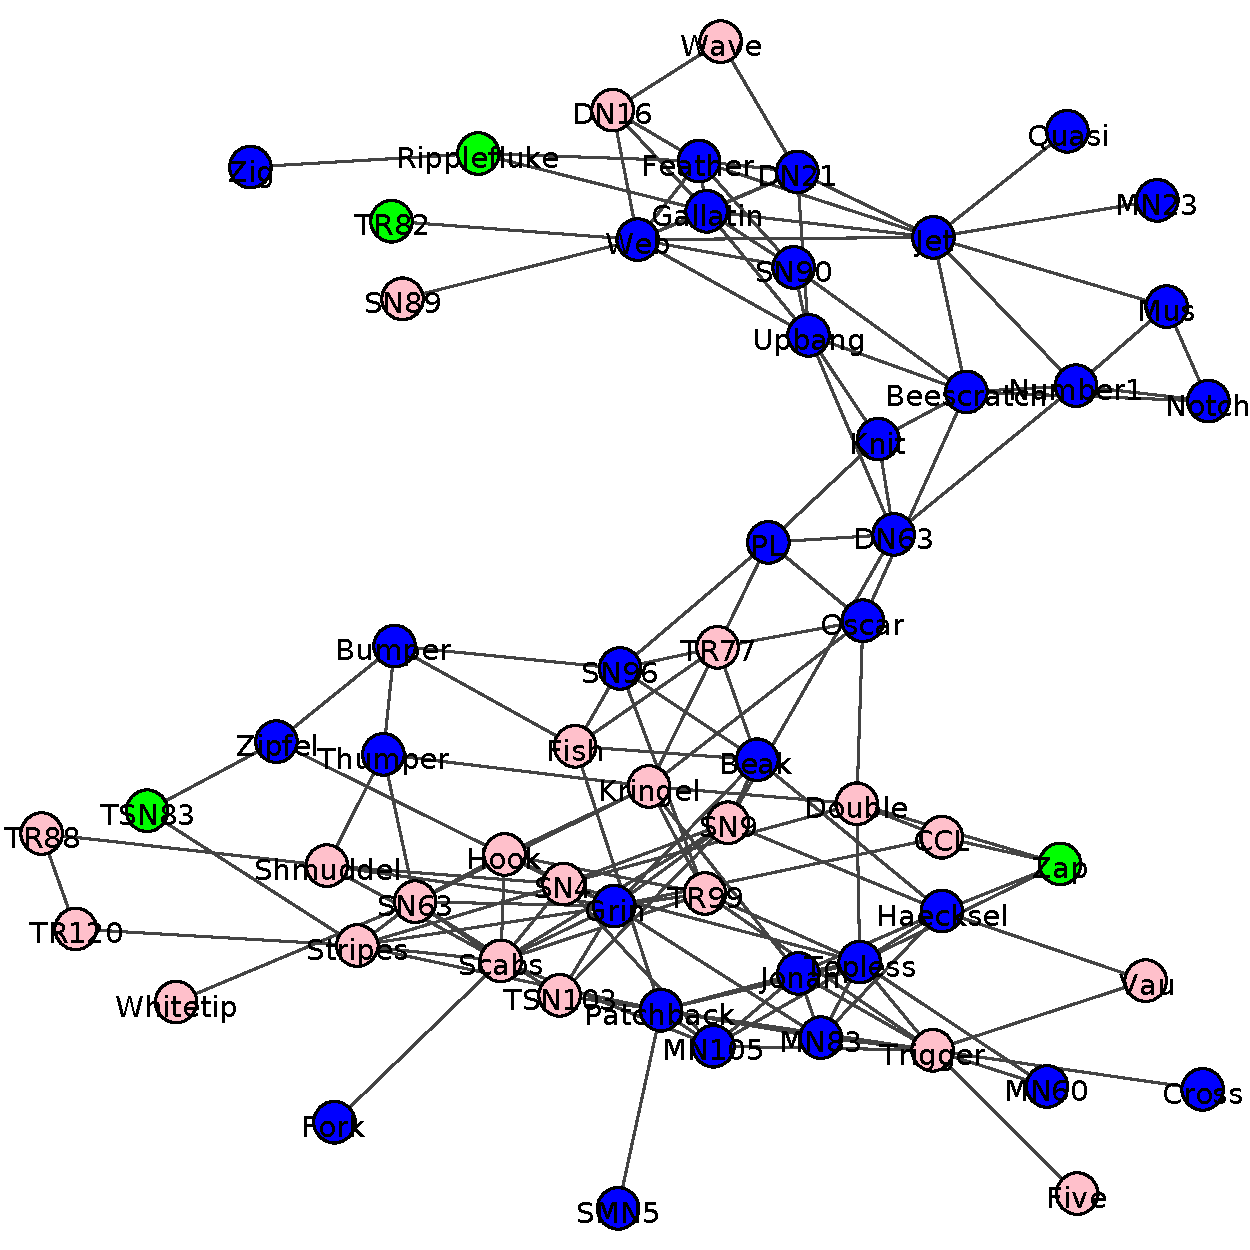
\includegraphics[scale = 0.27]{figuras/Parte_c0} 
}
\end{subfloat}
\begin{subfloat}[]
{
	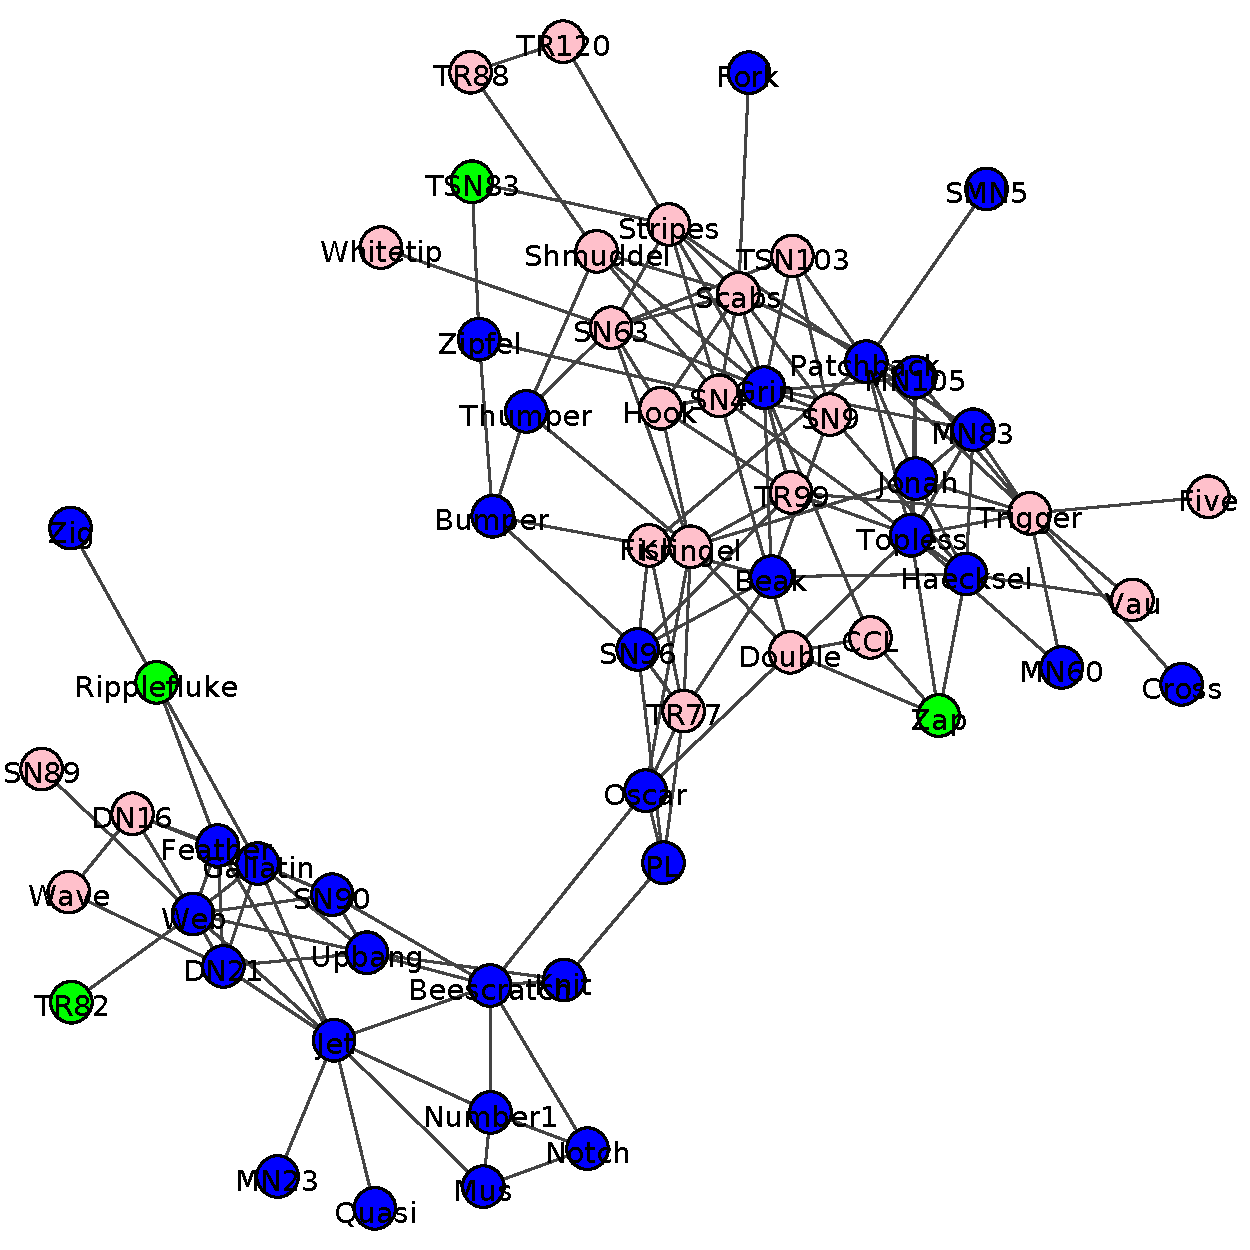
\includegraphics[scale = 0.27]{figuras/Parte_c1}
}
\end{subfloat}
\begin{subfloat}[]
{
	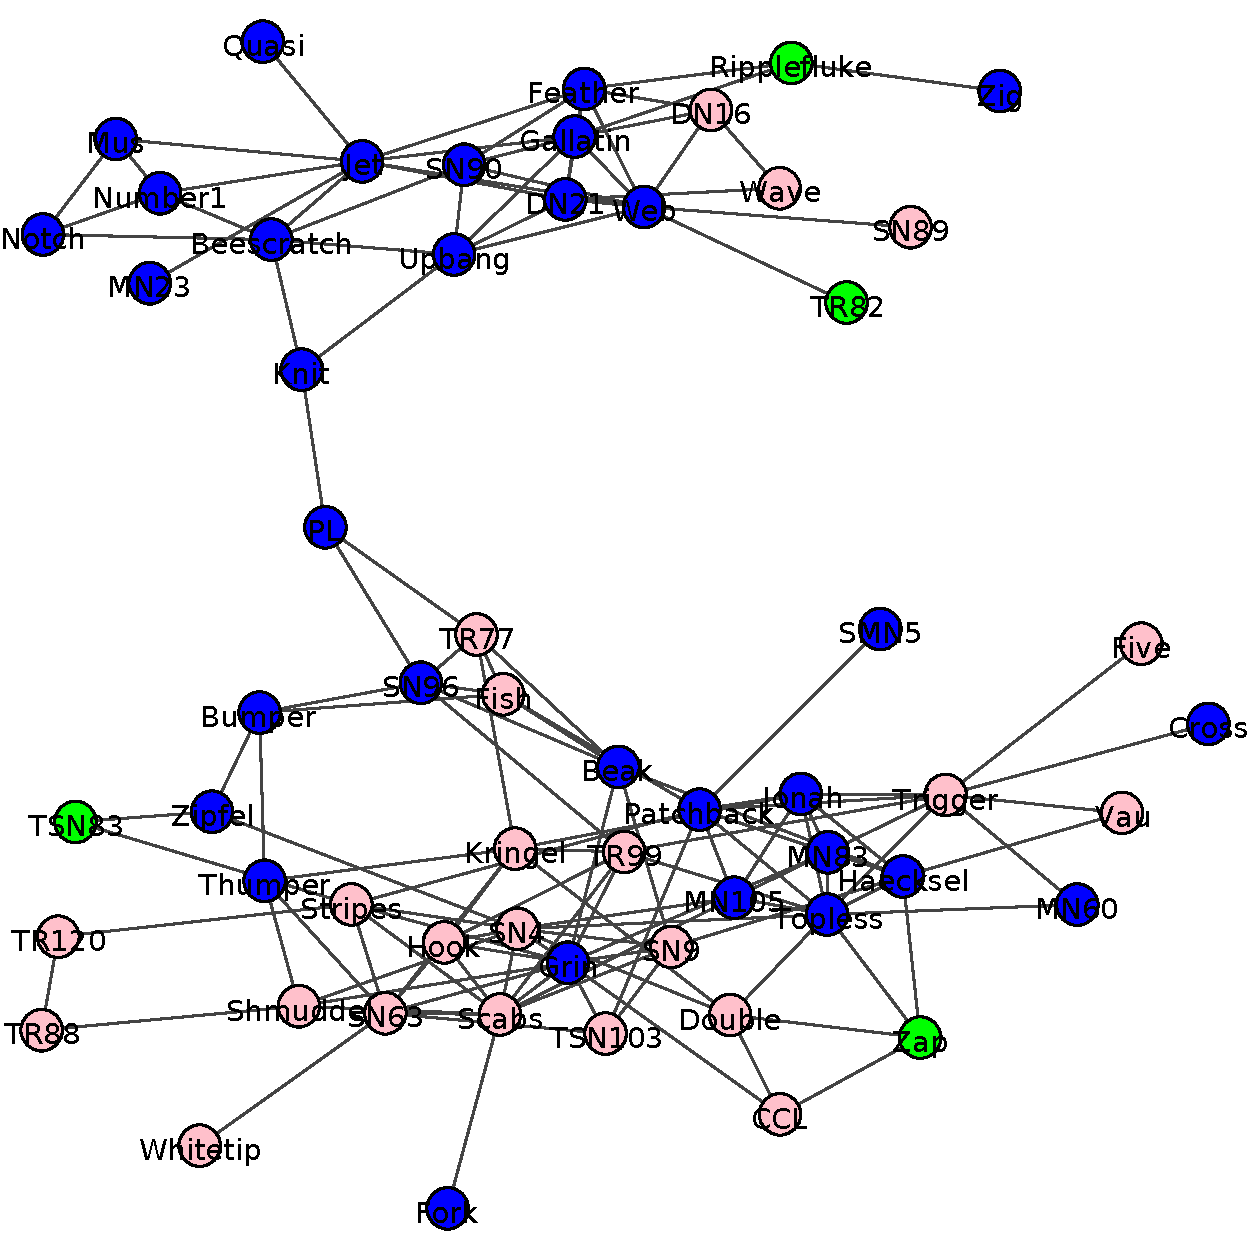
\includegraphics[scale = 0.27]{figuras/Parte_c2} 
}
\end{subfloat}
\begin{subfloat}[]
{
	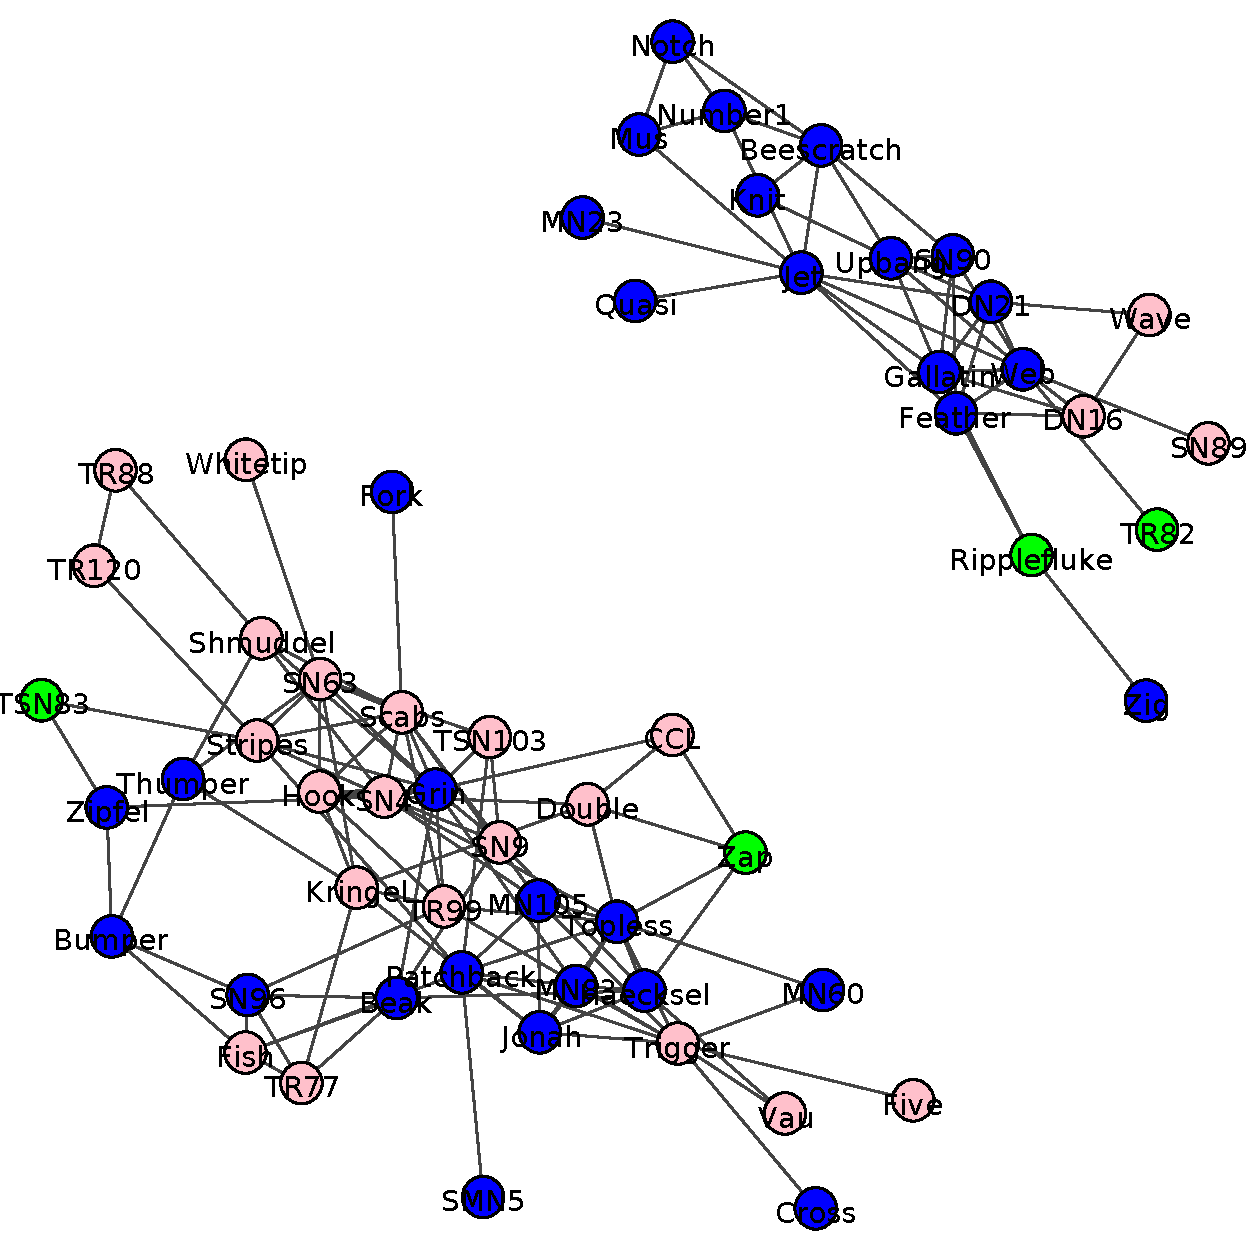
\includegraphics[scale = 0.27]{figuras/Parte_c3} 
}
\end{subfloat}
\label{fig:Betweennes}
\caption{Fruchterman - Reingold layout. Los colores de los nodos se refieren al sexo del delfín: azul, macho; rosa, hembra; verde, sexo no indicado en el dataset.}
\end{figure}

\newpage
%    \input{jimmy}
\newpage
    \section{Ejercicio 4}
La asortatividad/homofilia es la tendencia de un nodo, de una red, se conecte con otros 
de caracteristicas similares, esto en terminos mathematicos es evaluar la correlaci\'on
de links entre nodos del mismo tipo \citep{newman2003}. Esta propiedad tiende a ser caracteristica 
para tipos de redes distintas: En redes de amistad por ejemplo se tiende a hacer uniones entre
nodos \textit{parecidos}, mientras que en redes biologicas, los \textit{hubs} tienes a evadirse 
entre ellos y asociarse con nodos de menor grado \citep{newman,barabasi}. 

En este ejercicio se plantea evaluar la asortatividad de cuatro redes (dos sociales y dos biol\'ogicas) a trav\'es
de dos m\'etodos distintos: Mediante la estimaci\'on de la correlaci\'on de grado a partir del grado medio del
vecindario de un nodo \citep{barabasi}; y a trav\'es del Coeficiente de Correlaci\'on de Grado propuesto por Newman
\citep{newman2003,newman}.

\subsection{Consideraciones generales}
\begin{figure}[!ht]
    \centering
    \begin{subfigure}[b]{0.30\columnwidth}
        \includegraphics[width=\textwidth]{./schemes/netscience-gml.pdf}
        \caption{\label{fig4:NETSCIENCE}NETSCIENCE}
    \end{subfigure}
    \begin{subfigure}[b]{0.30\columnwidth}
        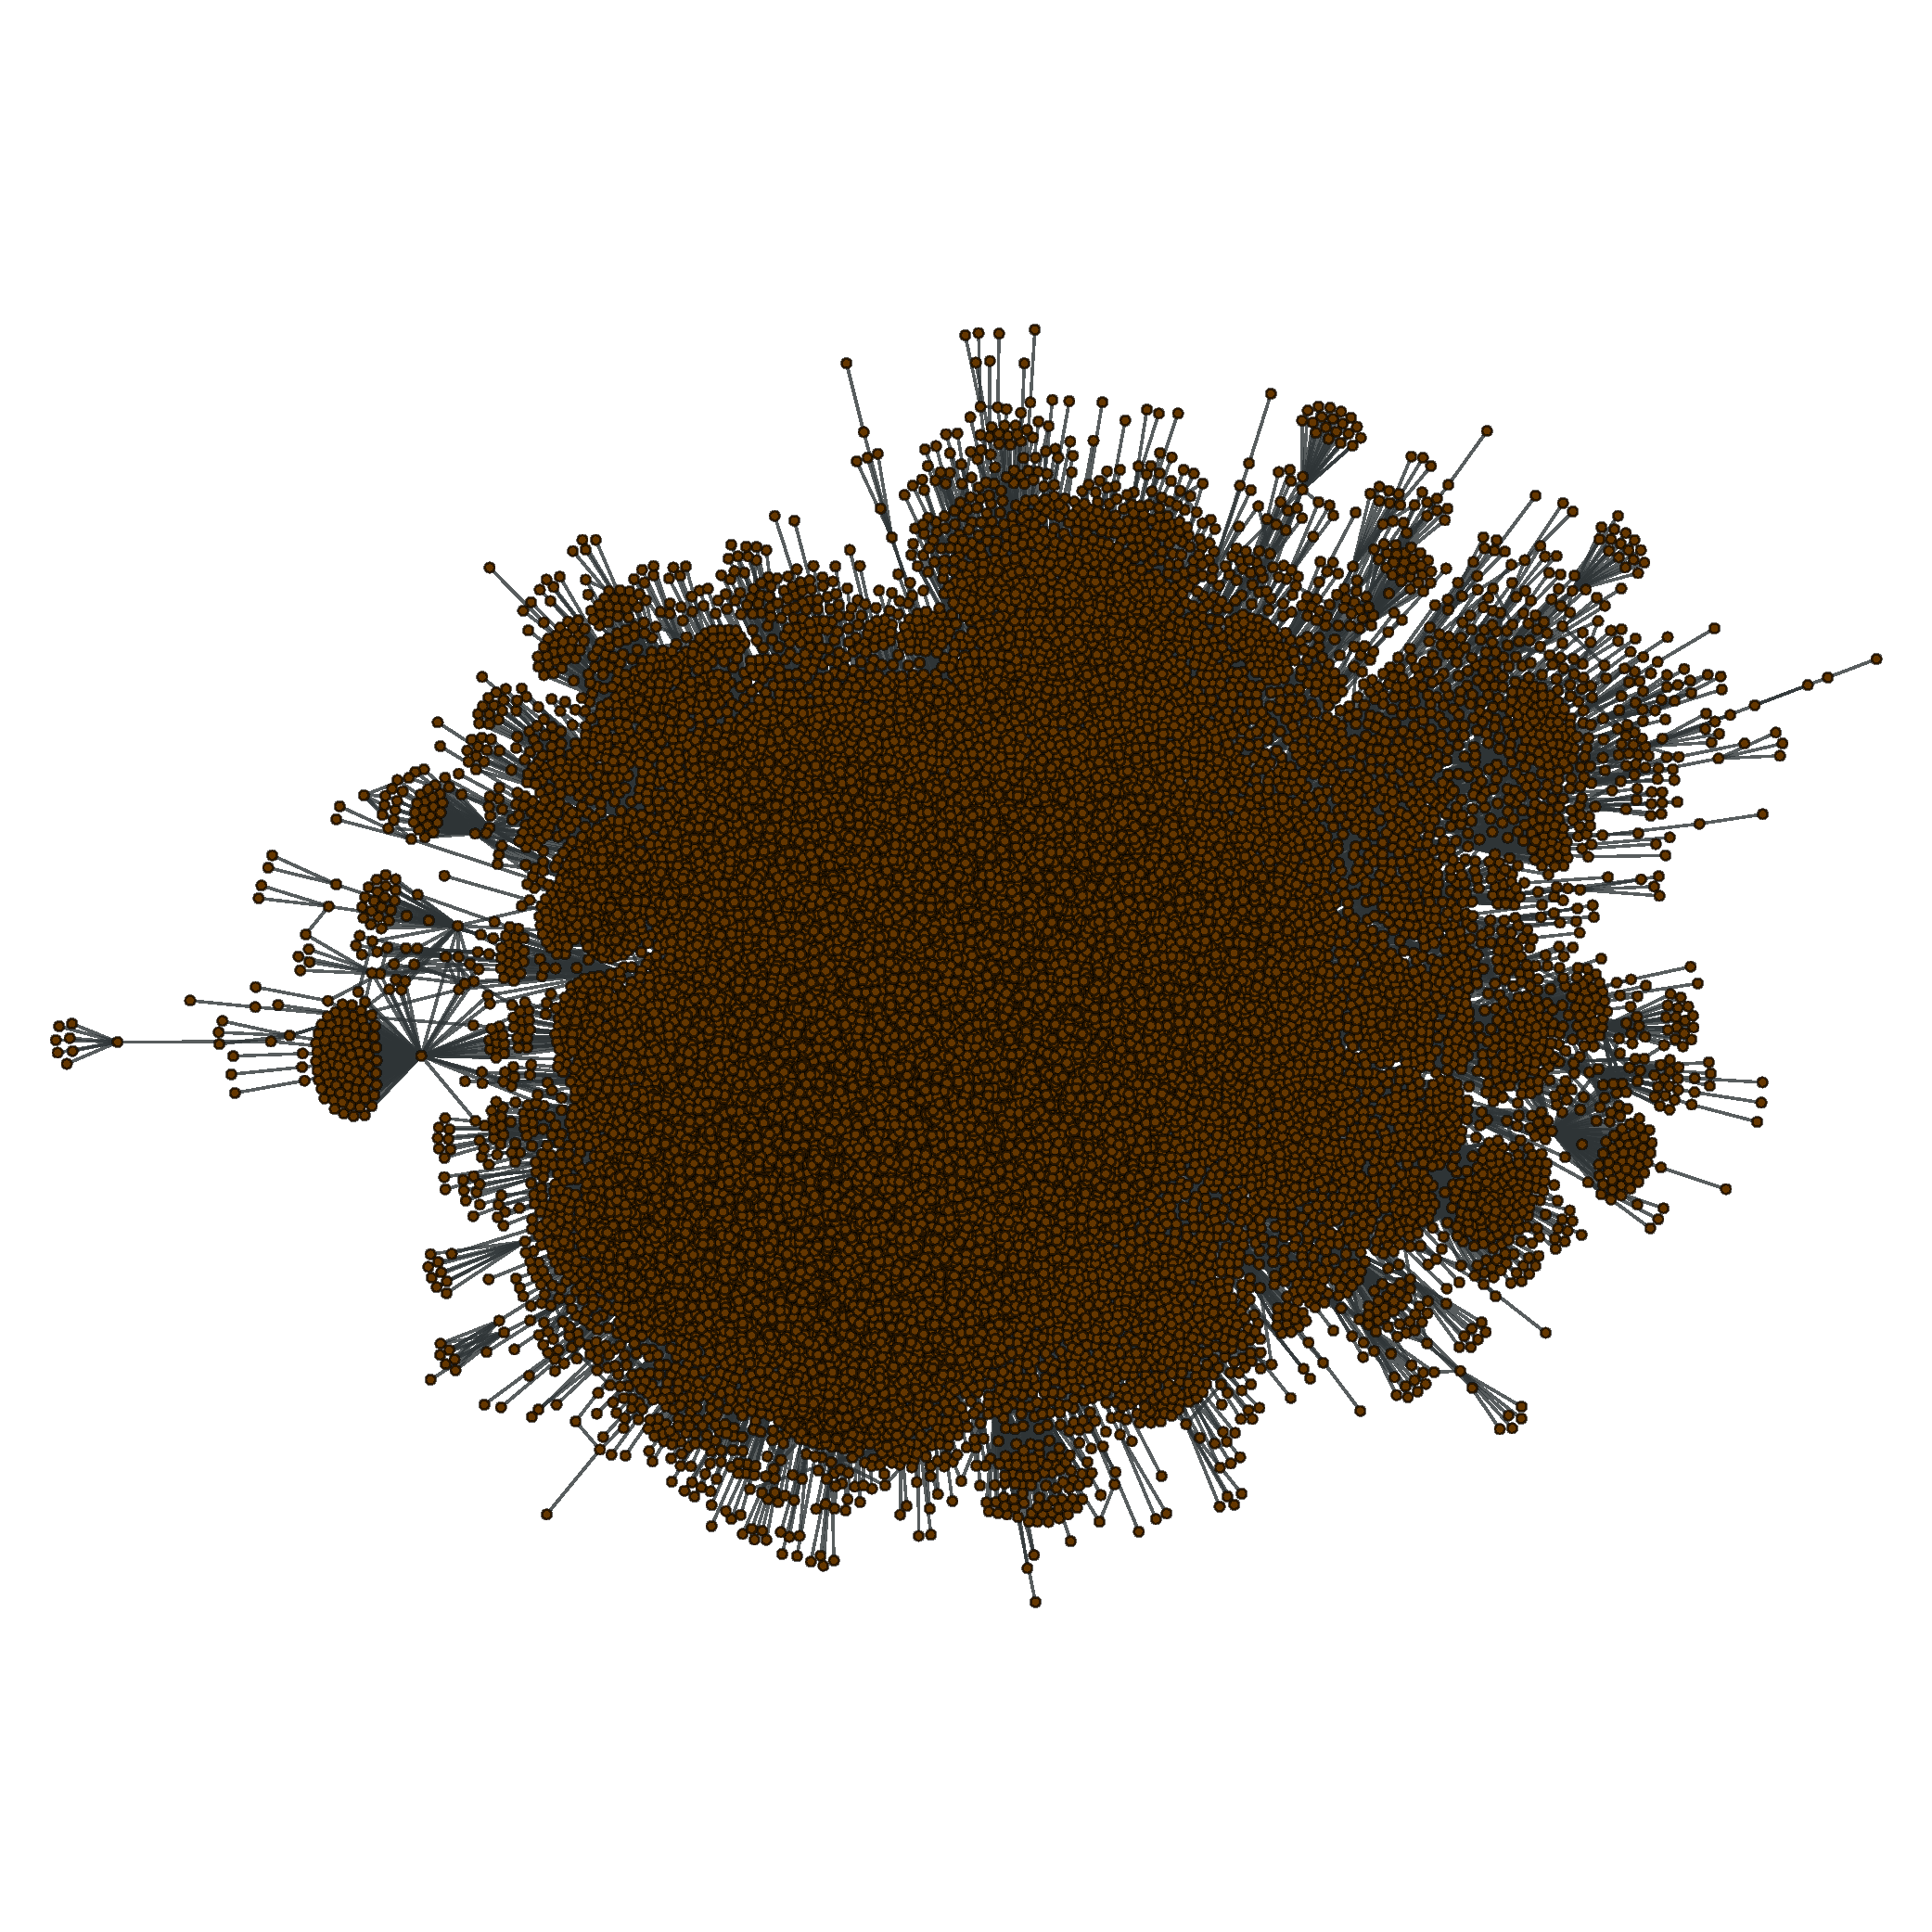
\includegraphics[width=\textwidth]{./schemes/as-22july06-gml.pdf}
        \caption{\label{fig4:WWW}WWW}
    \end{subfigure}
    \\
    \begin{subfigure}[b]{0.30\columnwidth}
        \includegraphics[width=\textwidth]{./schemes/yeast_AP-MS-txt.pdf}
        \caption{\label{fig4:ap_ms} AP-MS}
    \end{subfigure}
    \begin{subfigure}[b]{0.30\columnwidth}
        \includegraphics[width=\textwidth]{./schemes/yeast_Y2H-txt.pdf}
        \caption{\label{fig4:y2h} Y2H}
    \end{subfigure}
    \caption{\label{fig4:grafos}\textit{Layout} SFDP para cada red estudiada \\
    (script \texttt{plot.py~<archivo>\quad-f <fmt>}).}
\end{figure}
Consideremos las redes de colaboraciones cientificas (NETSCIENCE), red de internet (WWW) y dos redes de levadura analizadas 
en el ejercicio 1 (AP-MS y Y2H), las cuales son mostradas en la figura \ref{fig4:grafos}.


Un m\'etodo alternativo para 
evaluar asortividad es analizar la matriz de correlaci\'on entre grados (\textit{mixing matrix}) la cual se presenta en
la figura \ref{fig4:mix}.


\begin{figure}[!ht]
    \centering
    \begin{subfigure}[b]{0.45\columnwidth}
        \includegraphics[width=\textwidth]{./schemes/mixing_netscience-gml.pdf}
        \caption{\label{fig4:NETSCIENCE}NETSCIENCE}
    \end{subfigure}
    \begin{subfigure}[b]{0.45\columnwidth}
        \includegraphics[width=\textwidth]{./schemes/mixing_as-22july06-gml.pdf}
        \caption{\label{fig4:WWW}WWW}
    \end{subfigure}
    \\
    \begin{subfigure}[b]{0.45\columnwidth}
        \includegraphics[width=\textwidth]{./schemes/mixing_yeast_AP-MS-txt.pdf}
        \caption{\label{fig4:ap_ms} AP-MS}
    \end{subfigure}
    \begin{subfigure}[b]{0.45\columnwidth}
        \includegraphics[width=\textwidth]{./schemes/mixing_yeast_Y2H-txt.pdf}
        \caption{\label{fig4:y2h} Y2H}
    \end{subfigure}
    \caption{\label{fig4:mix} Mixing Matrix para cada caso. En la red WWW se ha ajustado los limites de gr\'afico
    de manera que sean visibles las correlaciones de bajo grado
    \\(script \texttt{degree\_mixing\_plot.py <archivo>\quad-f <fmt>})}
\end{figure}

De la figura se puede observar que, para todos los casos, la mayor densidad de correlaci\'on se puede encontrar en los 
grados peque\~nos, pero no es claro como se propaga esta correlaci\'on para grados mayores debido a que tiende rapidamente 
a cero. A\'un m\'as, no es posible hacer una comparaci\'on clara entre cada red a partir de sus respectivas matrices. Motivados por estas razones evaluamos otras m\'etodologias.

\subsection{Grado medio del vecindario $k_{nn}$ (revising \citet{barabasi})}
En esta metodolog\'ia estamos interesados en analizar el comportamiento de los vecinos de un nodo de grado $k$, para
ello consideramos el grado medio de los vecinos $k_{nn}$ de un nodo de grado $k$, esto es
\begin{align}
    k_{nn}(k) = \sum_{k'} k' P(k'|k)
\end{align}
este promedio est\'a hecho sobre la probabilidad de que: dado un nodo de grado $k$, tenga un vecino de grado $k'$.


\subsection{Coeficiente de Correlaci\'on de Grado}

\bibliographystyle{plainnat}
\bibliography{biblio}
\end{document}
